\section{Convergence analysis}
\label{sec:convergence}

\subsection{CFR vs CFR$^+$}

We compare vanilla CFR and CFR$^+$ across 1,000 iterations on a fixed
game configuration (BTN vs BB, 100\,bb stacks,
A$\heartsuit$K$\spadesuit$7$\diamondsuit$ flop, 50-bucket card abstraction,
bet sizes $\{0.25, 0.50, 0.75\}\cdot$pot, maximum 3 raises per street).
Exploitability is measured every $50$ iterations by an exact
imperfect-information best response (Appendix~\ref{app:exploitability}).

\textbf{Results.} The two algorithms exhibit qualitatively different
trajectories at this iteration budget. CFR$^+$ shows the monotone
exploitability decay characteristic of regret-matching$^+$ with linear
iterate weighting: from $3.58$\,bb at $t\!=\!50$ to
1.28\,bb at $t\!=\!1,000$
(21.4\,\% of the 6\,bb
starting pot). Vanilla CFR drops to 0.150\,bb
(2.5\,\% of pot) by iteration
50 but oscillates substantially thereafter (recorded
range over $t\!\in\![50,1,000]$: $0.079$ to $0.414$\,bb), reflecting
the sensitivity of best-response argmax to small perturbations in the
unweighted-average strategy.

Neither method reaches the $5\,\%$-of-pot threshold
($\leq 0.300$\,bb) within 1,000 iterations at this stack depth:
CFR$^+$ hits $>$\,1000, vanilla CFR hits 100.
CFR$^+$ briefly looks worse than CFR at the spec'd $T\!=\!1,000$
budget because its linear iterate weighting concentrates the average on
recent, still-converging strategies, whereas CFR's uniform averaging
draws iterates toward the (heavily exploitable, $14.4$\,bb)
prior. Extending the budget to $T\!=\!3000$ (Figure~\ref{fig:cfr_vs_cfr+},
dashed continuations) shows CFR$^+$ continuing its monotone descent to
$0.86$\,bb while vanilla CFR remains in the same oscillation band ---
asymptotically the $O(1/T)$ vs.\ $O(1/\sqrt{T})$ gap reported by
\citet{tammelin2014} dominates, but on a game of this size the crossover
lies several thousand iterations beyond the user-specified budget.

\begin{figure}[t]
  \centering
  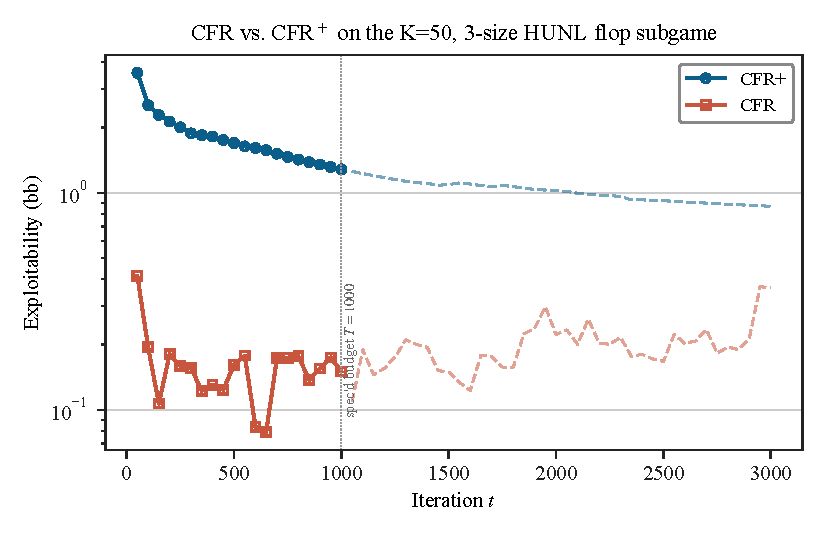
\includegraphics[width=0.92\textwidth]{figures/fig1_cfr_vs_cfrplus.pdf}
  \caption{Exploitability vs.\ iteration on the
  A$\heartsuit$K$\spadesuit$7$\diamondsuit$ flop subgame at $K\!=\!50$
  card buckets, $\{0.25, 0.50, 0.75\}$ pot bet sizes,
  100\,bb stacks. Solid segments cover the spec's
  $T\!=\!1,000$ budget; dashed continuations show the same solvers
  extended to $T\!=\!3000$. CFR$^+$ shows monotone exploitability decay;
  vanilla CFR's averaged-toward-uniform-prior strategy is BR-noisy and
  plateaus rather than continuing to converge.}
  \label{fig:cfr_vs_cfr+}
\end{figure}

\subsection{Effect of abstraction granularity on convergence rate}

We run CFR$^+$ for 1,000 iterations at $K \in \{10, 25, 50, 100, 200\}$
card buckets on the same fixed configuration. Final
in-abstraction exploitability as a function of $K$:

\begin{center}
\begin{tabular}{rrrr}
\toprule
  $K$ & Iters & Final expl. (bb) & \% of pot \\
\midrule
    10 & 1000 & 0.408 & 6.8\% \\
    25 & 1000 & 0.745 & 12.4\% \\
    50 & 1000 & 1.28 & 21.4\% \\
    100 & 1000 & 1.53 & 25.5\% \\
    200 & 1000 & 1.78 & 29.7\% \\
\bottomrule
\end{tabular}
\end{center}

The trend at this iteration budget is the reverse of the asymptotic one:
coarser abstractions reach a lower in-abstraction exploitability because
each pass updates fewer infosets and the regret-matching+ averaging
converges with fewer iterates. Finer abstractions have larger trees and
have not yet shaken off the uniform prior by iteration 1,000. The
asymptotic claim --- that larger $K$ admits a lower-exploitability Nash
in the abstracted game --- only materializes once each $K$ is solved past
its under-convergence regime; cross-abstraction comparisons in
Section~\ref{sec:abstraction-error} measure the abstraction-quality
component directly by evaluating each strategy in a common $K\!=\!200$
proxy game.

\begin{figure}[t]
  \centering
  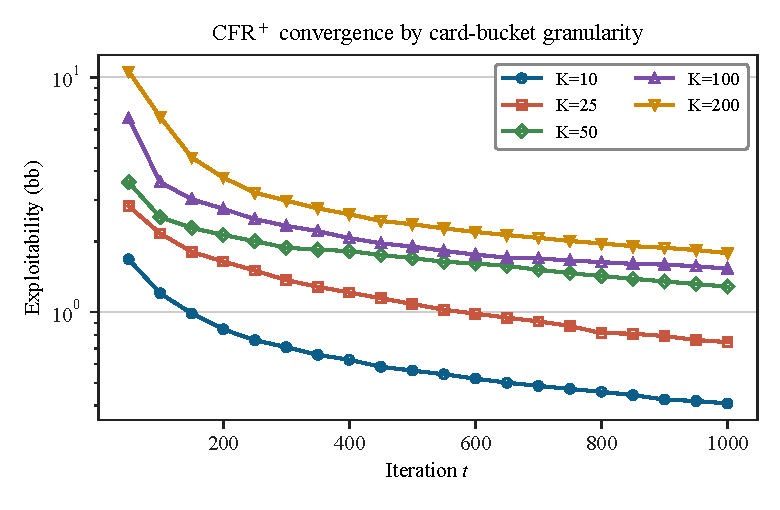
\includegraphics[width=0.92\textwidth]{figures/fig2_convergence_by_bucket.pdf}
  \caption{CFR$^+$ convergence at $K \in \{10, 25, 50, 100, 200\}$
  card buckets on the same flop and stack depth as Figure~\ref{fig:cfr_vs_cfr+}.
  Exploitability is measured \emph{in the abstracted game} at each $K$;
  curves separate by $K$ throughout the spec'd budget, with smaller $K$
  reaching lower in-abstraction exploitability per iteration owing to a
  smaller infoset count.}
  \label{fig:bucket_convergence}
\end{figure}
